\chapter{Analysis}

\section[Reelle Zahlen]{Reelle Zahlen $\boldsymbol{\mathbb{R}}$}

\subsection{Angeordnete Körper}
\index{Angeordnete Körper}

(Gilt auch für $\mathbb{Z}$ und $\mathbb{Q}$)

\paragraph{Körperaxiome $\mathbf{(\mathbb{R}, +, *)}$}
\index{Körperaxiome}
$a,b,c \in \mathbb{R}$

\begin{description}
  \item [Addition $(\mathbb{R},+)$]
        \index{Addition}\
        \begin{description}
          \item [Assoziativität]
                \index{Assoziativität}
                $\linebreak a + (b + c) = (a + b) + c$

          \item [Kommutativität]
                \index{Kommutativität}
                $\linebreak a + b = b + a$

          \item [Neutrales Element Null]
                \index{Null}
                $\linebreak a + 0 = a \quad 0 \in \mathbb{R}$

          \item [Inverses ,,Negativ``]
                \index{Negatives}
                $\linebreak a + (-a) = 0 \quad (-a) \in \mathbb{R}$
        \end{description}

  \item [Multiplikation $(\mathbb{R},*)$]\
        \index{Multiplikation}
        \begin{description}
          \item [Assoziativität]
                \index{Assoziativität}
                $a * (b * c) = (a * b) * c$

          \item [Kommutativität]
                \index{Kommutativität}
                $a * b = b * a$

          \item [Neutrales Element Eins]
                \index{Eins}
                $\linebreak a * 1 = a \quad 1 \in \mathbb{R} \setminus \{ 0 \}$

          \item [Inverses ,,Kehrwert``]
                \index{Kehrwert}
                $\linebreak a * (a^{-1}) = 1$ \\
                $a \boldsymbol{\neq} \mathbf{0}, (a^{-1}) \in \mathbb{R}$
        \end{description}
  \item [Distributivität]
        \index{Distributivität}
        $\linebreak \mathbf{a} * (b + c) = \mathbf{a} * b + \mathbf{a} * c$
\end{description}

\paragraph{Totale Ordnung}

\begin{description}
  \item [Transitivität]
        \index{Transitivität der Ordnung}
        $\linebreak a < b \land b < c \Rightarrow a < c$

  \item [Trichotomie] Entweder \\
        \index{Trichotomie}
        \index{Irreflexivität der Ordnung}
        $a < b$ oder $a = b$ oder $b < a$ \\
        $\Rightarrow$ \emph{Irreflexivität} ($a < b \Rightarrow a \neq b$)

  \item [Addition]
        $\linebreak a < b \Rightarrow a + c < b + c$

  \item [Multiplikation]
        $\linebreak a < b \Rightarrow a * c < b * c \quad 0 < c$
\end{description}

% % Korrelat
% \paragraph{Notation}
% 
% \begin{align*}
%   a > b    & :\Leftrightarrow b < a            \\
%   a \leq b & :\Leftrightarrow a < b \lor a = b \\
%   a \geq b & :\Leftrightarrow a > b \lor a = b
% \end{align*}
% 
% \paragraph{Lemma}
% 
% \begin{itemize}
%   \item $a \leq a$
%   \item $a < b \Rightarrow a \neq b$
%   \item $a \leq b \lor b \leq a$
%   \item $a \leq b \land b \leq a \Rightarrow a = b$
%   \item $a < b \Rightarrow a * c \boldsymbol{>} b * c \quad 0 < c$
%   \item $a < b \land c < d \Rightarrow a + c < b + d$
%   \item $c < 0 \Leftrightarrow - c > 0$
%   \item $a \neq 0 \Rightarrow a^2 > 0$
%   \item $a < 0 \Rightarrow a^{-1} < 0$
%   \item $0 < a < b \Rightarrow b^{-1} < a^{-1}$
% \end{itemize}

Bei Additiver oder Multiplikativer Inversion dreht sich die Ungleichung.

\subsection{\textsc{Archimedes} Axiom}
\index{\textsc{Archimedes} Axiom}

\begin{align*}
  \forall x \in \mathbb{R} \exists n \in \mathbb{N}: & n > x           \\
                                                     & n > \frac{1}{x}
\end{align*}

\subsection{Teilbarkeit}
\index{Teilbarkeit}

$$a | b \Leftrightarrow \exists n \in \mathbb{Z}: b = a * n$$

($\Rightarrow \sqrt{2} \notin \mathbb{Q}$, da mit $\frac{a}{b} = \sqrt{2}$ nicht teilerfremd)
\index{Irrationalität}

\subsection{Häufige Fehler}

\begin{itemize}
  \item Nicht durch Null teilen/kürzen

  \item Nicht $-x < 0$ annehmen

  \item Multiplikation mit negativen Zahlen kehrt Ungleichungen
\end{itemize}

\subsection{Operationen}

\paragraph{Brüche}
\index{Bruch}

\begin{itemize}
  \item $\frac{a}{b} * \frac{c}{d} = \frac{a * c}{b * d}$

  \item $\frac{a}{b} \overset{\mathbf{* d}}{=} \frac{a \mathbf{* d}}{b \mathbf{* d}}$

  \item $\frac{a}{\mathbf{c}} + \frac{b}{\mathbf{c}} = \frac{a + b}{\mathbf{c}}$

  \item $\frac{a}{b} + \frac{c}{d} = \frac{a * d + c * b}{b * d}$
\end{itemize}

\paragraph{Wurzeln} $b^n = a \Leftrightarrow b = \sqrt[n]{a}$
\index{Wurzel}

\begin{itemize}
  \item $\sqrt[n]{\mathbf{a * b}} = \sqrt[n]{\mathbf{a}} \mathbin{\boldsymbol{*}} \sqrt[n]{\mathbf{b}}$

  \item $\sqrt[\mathbf{n}]{ \sqrt[\mathbf{m}]{a} } = \sqrt[\mathbf{n * m}]{a}$

  \item $\sqrt[n]{a} < \sqrt[n]{b} \quad 0 \leq a < b$

  \item $\sqrt[n+1]{a} < \sqrt[n]{a} \quad 1 < a$

  \item $\sqrt[n]{a} < \sqrt[n+1]{b} \quad 0 < a < 1$
\end{itemize}

$$\sqrt[n]{a^n} = |a| \quad a \in \mathbb{R}$$

\paragraph{Potenzen} $a^{\frac{x}{y}} = \sqrt[y]{a^x}$
\index{Potenz}

\begin{itemize}
  \item $a^{\mathbf{x}} * b^{\mathbf{x}} = (a \mathbf{*} b)^{\mathbf{x}}$

  \item $a^x * a^y = a^{x \boldsymbol{+} y}$

  \item $(a^x)^y = a^{x \boldsymbol{*} y}$

        % \item $a^x < a^y \quad 1 < a, x < y$
        % \item $a^x > a^y \quad 0 < a < 1, x < y$
        % \item $a^x < b^x \quad a < b, 0 < x$
        % \item $a^x > b^x \quad a < b, x < 0$
\end{itemize}

\section{Intervalle}
\index{Intervall}

Sei $A \subseteq \mathbb{R}, A \neq \emptyset, a_0 \boldsymbol{\in} A$.

\begin{description}
  \item [Geschlossen]
        \index{Abgeschlossen}
        $[a;b] := \{ x \in \mathbb{R} \mid a \boldsymbol{\leq} x \boldsymbol{\leq} b \}$ \\
        (,,Ecken sind mit enthalten``)

  \item [Offen]
        \index{Offen}
        $(a;b) := \{x \in \mathbb{R} \mid a \boldsymbol{<} x \boldsymbol{<} b\}$ \\
        (Bei $\infty$ immer offen, da $\infty \notin \mathbb{R}$)
\end{description}

\paragraph{Kleinstes/Grö\ss tes Element}

\begin{description}
  \item [Minimum]
        \index{Minimum}
        $\min(A) := a_0$ \\
        $\Leftrightarrow \forall a \in A: \mathbf{a_0} \boldsymbol{\leq} a$

  \item [Maximum]
        \index{Maximum}
        $\max(A) := a_0$ \\
        $\Leftrightarrow \forall a \in A: \mathbf{a} \boldsymbol{\leq} a_0$
\end{description}

($\nexists {}^{\min}/_{\max} (a;b)$)

\paragraph{Beschränktheit} $A$ hei\ss t
\index{Beschränkte Menge}

\begin{description}
  \item [Oben beschränkt]
        \index{Obere Schranken}
        $\exists s \in \mathbb{R} \forall a \in A: \mathbf{a} \boldsymbol{\leq} s$

  \item [Unten beschränkt]
        \index{Untere Schranken}
        $\exists s \in \mathbb{R} \forall a \in A: \mathbf{s} \boldsymbol{\leq} a$
\end{description}

\paragraph{Vollständigkeit}
\index{Vollständigkeit}

\begin{description}
  \item [Infimum (klein)] $\inf(A)$ \\
        \index{Infimum}
        $:= \mathbf{\max} \{ s \in \mathbb{R} \mid \forall a \in A: \mathbf{s} \boldsymbol{\leq} a \}$

  \item [Supremum (gro\ss)] $\sup(A)$ \\
        \index{Supremum}
        $:= \mathbf{\min} \{ s \in \mathbb{R} \mid \forall a \in A: \mathbf{a} \boldsymbol{\leq} s \}$
\end{description}

\paragraph{Vollständigkeitsaxiom} $\exists \sup(A)$.
\index{Vollständigkeitsaxiom}

\mzGraphic{
  \begin{tikzpicture}
    \draw[->] (-3,0) -- (4,0);

    \draw
    (0,0) node[above=1.5] (interval) {$A$}

    (0,0) + (-1,0) node (links) {$[$}
    (0,0) + (1,0) node (rechts) {$]$}

    (links.north) node[above right] {$\min$}
    (links.west) node[below left] {$\inf$}

    (links.west) + (-1,0) node[above left] {\shortstack{Untere\\Schranken}}

    (rechts.north) node[above left] {$\max$}
    (rechts.east) node[below right] {$\sup$}

    (rechts.east) + (1,0) node[above right] {\shortstack{Obere\\Schranken}}

    (4,0) node[below right] {$\mathbb{R}$};

    \draw[color=primary,decorate,decoration=coil]
    (links) -- (rechts);
  \end{tikzpicture}
}

\section{Folgen}

\paragraph{Folge $\mathbf{(a_n)_{n \in \mathbb{N}}}$} in $A$ ist eine Abb. $f: \mathbb{N} \rightarrow A$ mit $a_n = f(n)$.
\index{Folge}

\begin{description}
  \item [Arithmetische Folge]
        \index{Arithmetische Folge}
        $a_{n+1} = a_n + d$ \\
        $a_n = a + (n-1) * d \quad d, a \in \mathbb{R}$

  \item [Geometrische Folge]
        \index{Geometrische Folge}
        $a_{n+1} = a_n * q$ \\
        $a_n = q^n \quad q \in \mathbb{R}$
\end{description}

\paragraph{Rekursion} $a_n$ ist auf $\mathbf{a_{n-1}}$ definiert.
\index{Rekursion}

\begin{align*}
  a_{n+1} = & F(n, a_n) \quad \forall n \in \mathbb{N} \\
            & F: A \times \mathbb{N} \rightarrow A
\end{align*}

\paragraph{Primfaktorzerlegung} $n\in \mathbb{N}, n \geq 2$
\index{Primfaktorzerlegung}

$$\exists p_1, \dots, p_n \in \mathbb{P}: n = \mathbf{p_1 * \cdots * p_n}$$

\subsection{Summen und Produkte}

\begin{description}
  \item [Summe] $\sum_{i = 1}^n i = 1 + 2 + \cdots + n$
        \index{Summ}

  \item [Produkt] $\prod_{i = 1}^n i = 1 * 2 * 3 * \cdots * n$
        \index{Produkt}

  \item [Fakultät] $n! = \prod^n i$ ($\mathbf{0! = 1}$)
        \index{Fakultät}
\end{description}

\paragraph{\textsc{Gaussche} Summe} $n \in \mathbb{N}$
\index{\textsc{Gaussche} Summenformel}

$$\sum^n i = \frac{n * (n + 1)}{2}$$

\paragraph{Geom. Summe} $q \in \mathbb{R} \ \{ 0 \}, n \in \mathbb{N}_0$
\index{Geometrische Summe}

$$\sum_{i=0}^n q^i = \frac{1 - q^{n+1}}{1 - q}$$

\paragraph{\textsc{Bernoulli} Unglei.} $n \in \mathbb{N}_0, x \geq -1$
\index{\textsc{Bernoulli} Ungleichung}

$$(1 + x)^n \geq 1 + n * x$$

\paragraph{Binom. Koeff.} $\binom{n}{k} = \frac{n!}{k! * (n - k)!}$
\index{Binomial Koeffizient}

\begin{itemize}
  \item Rechnen: $\frac{n > k}{0 < (n - k)}$

  \item $\binom{n}{0} = \binom{n}{n} = 1$

  \item $\binom{n + 1}{k + 1} = \binom{n}{k} + \binom{n}{k + 1}$
\end{itemize}

\paragraph{Binomischer Satz} $n \in \mathbb{N}$
\index{Binomischer Satz}

$$(a + b)^n = \sum_{k=0}^n \binom{n}{k} * a^{n - k} * b^k$$

\section{Grenzwerte}

\paragraph{Betrag} $|x| := \begin{cases}
      & x \quad 0 \leq x \\
    - & x \quad x < 0    \\
  \end{cases}$
\index{Betrag}

\begin{description}
  \item [Lemma] $|x * y| = |x| * |y|$

  \item [Dreiecksungleichung]
        \index{Dreiecksungleichung}
        $|x + y| \boldsymbol{\leq} |x| + |y|$

  \item [Umgekehrte \linebreak Dreiecksungleichung]
        \index{Umgekehrte Dreiecksungleichung}
        $\linebreak ||x| - |y|| \leq |x - y|$
\end{description}

\subsection{Konvergenz}
\index{Konvergenz}

Sei $(a_n)_{n \in \mathbb{N}} \subseteq \mathbb{R}, a \in \mathbb{R}$.

\begin{gather*}
  a_n \xrightarrow{n \rightarrow \infty} a \Leftrightarrow \\
  \forall \epsilon > 0 \exists n_0 \in \mathbb{N} \forall n \in \mathbb{N} n \geq n_0: \\
  \mathbf{|a_n - a| \leq \epsilon} \\
  (a - \epsilon \leq a_n \leq a + \epsilon)
\end{gather*}

\mzScale{0.5}{
  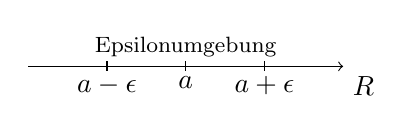
\begin{tikzpicture}
    \draw[->] (-2,0) -- (2,0) node[below right] {$\mathbb{R}$};

    \node at (0,0) (a) [below] {$a$};
    \node at (-1,0) (minus) [below] {$a - \epsilon$};
    \node at (1,0) (plus) [below] {$a + \epsilon$};

    \node at (a.north) [above] {\footnotesize Epsilonumgebung \index{Epsilonumgebung}};

    \draw (a.north) + (0,1/16) -- +(0,-1/16)
    (minus.north) + (0,1/16) -- +(0,-1/16)
    (plus.north) + (0,1/16) -- +(0,-1/16);
  \end{tikzpicture}
}

\begin{itemize}
  \item $a_n \xrightarrow{n \rightarrow \infty} a \Leftrightarrow \boldsymbol{\lim}_{n \rightarrow \infty} a_n = a$
        \index{Limes}
\end{itemize}

Beschränkt + monoton $\Rightarrow$ konvergent:

$$\lim_{n \rightarrow \infty} a_n = \begin{cases}
    \boldsymbol{\inf} \{ a_n \mid n \in \mathbb{N} \} \quad (a_n)_\text{\emph{fall.}} \\
    \boldsymbol{\sup} \{ a_n \mid n \in \mathbb{N} \} \quad (a_n)_\text{\emph{steig.}}
  \end{cases}$$

\begin{description}
  \item [Nullfolgen] $\lim_{n \rightarrow \infty} a_n = \mathbf{0}$
        \index{Nullfolge}
        \begin{itemize}
          \item  $\lim_{n \rightarrow \infty} \frac{1}{n^k} = \mathbf{0} \quad k \in \mathbb{N}$

          \item $\lim_{n \rightarrow \infty} n * q^n = \mathbf{0}$
        \end{itemize}

        \item[Folgen gegen $\mathbf{1}$]\
        % \index{Folge gegen Eins}

        \begin{itemize}
          \item $\lim_{n \rightarrow \infty} \sqrt[n]{a} = \mathbf{1} \quad a > 0$

          \item $\lim_{n \rightarrow \infty} \sqrt[n]{n} = \mathbf{1}$
        \end{itemize}

\end{description}

\paragraph{Bestimmt Divergent}
\index{Bestimmt Divergent}

\begin{gather*}
  a_n \xrightarrow{n \rightarrow \infty} \boldsymbol{\infty} \Leftrightarrow \\ \forall R \boldsymbol{>} 0 \exists n \geq n_0 \in \mathbb{N}: a_n \boldsymbol{\geq} R \\
  a_n \xrightarrow{n \rightarrow \infty} \boldsymbol{-\infty} \Leftrightarrow \\ \forall R \boldsymbol{<} 0 \exists n \geq n_0 \in \mathbb{N}: a_n \boldsymbol{\leq} R
\end{gather*}

$$
  \lim_{n \rightarrow \infty} q^n \begin{cases}
    = \mathbf{0} \quad         & (-1; 1) \\
    = \mathbf{1} \quad         & = 1     \\
    \geq \mathbf{\infty} \quad & > 1     \\
    \mathbf{\text{div.}} \quad & \leq -1
  \end{cases}
$$

\paragraph{Monotonie} % $(a_n)_{n \in \mathbb{N}} \subseteq \mathbb{R}$
\index{Monotonie}

\begin{description}
  \item [Monoton fallend]
        \index{Monton fallend}
        $\linebreak a_n \underset{\text{(streng)}}{\boldsymbol{\geq}} a_{n + 1} \quad \forall n \in \mathbb{N}$

  \item [Monoton steigend]
        \index{Monoton steigend}
        $\linebreak a_n \underset{\text{(streng)}}{\boldsymbol{\leq}} a_{n + 1} \quad \forall n \in \mathbb{N}$
\end{description}

\paragraph{Beschränktheit} % $(a_n)_{n \in \mathbb{N}} \subseteq \mathbb{R}$
\index{Beschränkte Folge}

$$\exists k > 0 \forall n \in \mathbb{N}: \mathbf{|a_n| \leq k}$$

\begin{itemize}
  \item Konvergent $\Rightarrow$ beschränkt

  \item Unbeschränkt $\Rightarrow$ divergent
\end{itemize}

\section{Grenzwertsätze}
\index{Grenzwertsätze}

$$\lim_{n \rightarrow \infty} a_n = a, \lim_{n \rightarrow \infty} b_n = b$$

\begin{itemize}
  \item $a_n \xrightarrow{n \rightarrow \infty} a \land a_n \xrightarrow{n \rightarrow \infty} b \linebreak \Rightarrow a = b$ (Max. einen Grenzw.)

  \item $a = \mathbf{0} \land (b_n)_\text{\emph{beschr.}}$ \\
        $\Leftrightarrow \lim_{n \rightarrow \infty} a_n * b_n = \mathbf{0}$

  \item $a_n \boldsymbol{\leq} b_n \Leftrightarrow a \boldsymbol{\leq} b \quad (\text{nicht} <)$

  \item
        $\lim_{n \rightarrow \infty} \begin{cases}
            a_n \boldsymbol{\pm} b_n = a \boldsymbol{\pm} b                                                   \\
            a_n \boldsymbol{\divideontimes} b_n = a \boldsymbol{\divideontimes} b                             \\
            a_n \boldsymbol{*} c = a \boldsymbol{*} c                                                         \\
            \mathbf{\sqrt[\color{black}k]{\color{black}a_n}} = \mathbf{\sqrt[\color{black}k]{\color{black}a}} \\
            \boldsymbol{|}a_n\boldsymbol{|} = \boldsymbol{|}a\boldsymbol{|}
          \end{cases}$
\end{itemize}

\paragraph{Einschachtelungssatz}
\index{Einschachtelungssatz}
\index{Sandwichtheorem}

\begin{gather*}
  \lim_{n \rightarrow \infty} a_n = \lim_{n \rightarrow \infty} b_n = a \\
  \forall n \geq N \in \mathbb{N}: \mathbf{a_n \leq c_n \leq b_n} \\
  (\exists) \lim_{n \rightarrow \infty} c_n = \mathbf{a}
\end{gather*}

\subsection{Spezielle Folgen}

\index{Teilfolge}
\paragraph{Teilfolge} \emph{streng mnt.} Folge $(b_k)_{n \in \mathbb{N}}$ mit $(n_k)_{k \in \mathbb{N}}$, sodass $b_k = \mathbf{{a_n}_k} \quad \forall k \in \mathbb{N}$.

$$\lim_{n \rightarrow \infty} a_n = a \Rightarrow \lim_{n \rightarrow \infty} {a_n}_k = a$$

(da $n_k$ mnt. steigend)

$$\forall (a_n)_{n \in \mathbb{N}} \exists {({a_n}_k)_{k \in \mathbb{N}}}_\text{\emph{mnt.}}$$

(nicht streng!)

\paragraph{Häufungspunkt} $h$ mit einer Teilfolge
\index{Häufungspunkt}

$$\lim_{n \rightarrow \infty} {a_n}_k = h$$

\begin{itemize}
  \item $\lim_{n \rightarrow \infty} a_n = a \Leftrightarrow \exists!: h = a$
\end{itemize}

\paragraph{\textsc{Bolzano-Weierstra\ss}}
\index{\textsc{Bolzano-Weierstra\ss}}

$${(a_n)_{n \in \mathbb{N}}}_{\text{\emph{beschr.}}} \Rightarrow \exists h_\text{\emph{Häuf.}}$$

(Teilfolge + (beschr.) $\Rightarrow \exists$ Häuf.)

\subsection{Cauchy-Folge}
\index{Cauchy-Folge}

\begin{gather*}
  \forall \epsilon > 0 \exists n_0 \in \mathbb{N} \forall n, m \geq n_0:\\
  |a_n - a_m| \leq \epsilon
\end{gather*}

(Konv. ohne bekannten Grenzwert)

\paragraph{Vollständigkeit von $\boldsymbol{\mathbb{R}}$}
\index{Vollständigkeit der Reelen Zahlen}

$${(a_n)_{n \in \mathbb{N}}}_\text{\emph{Cauchy}} \Leftrightarrow \exists \lim_{n \rightarrow \infty} a_n$$

\begin{align*}
  (\exists \lim_{n \rightarrow \infty} a_n
   & \Rightarrow {(a_n)_{n \in \mathbb{N}}}_\text{Cauchy}  \\
   & \Rightarrow {(a_n)_{n \in \mathbb{N}}}_\text{beschr.} \\
   & \Rightarrow \exists h \quad \text{\tiny (BW)}         \\
   & \Rightarrow \lim_{n \rightarrow \infty} a_n = h)
\end{align*}

\section{Reihen}

\begin{description}
  \item [Reihe $(s_n)_{n \in \mathbb{N}} = \sum_{k=1}^\infty a_k$]
        \index{Reihe}
        mit den Gliedern $(a_k)_{k \in \mathbb{N}}$.

  \item [$n$te Partialsumme]
        \index{Partialsumme}
        $s_n = \sum_{k=1}^{\mathbf{n}} a_k$

  \item [Grenzwert] ebenfalls $\sum_{k=1}^\infty a_k$, falls $s_n$ konvergiert
\end{description}

\paragraph{Spezielle Reihen}

\begin{description}
  \item[Geom.]
    \index{Geometrische Reihe}
    $\sum_{k=0}^\infty q^k = \frac{1}{1- q} \quad q \in (-1;1)$

  \item [Harmon.]
        \index{Geometrische Reihe}
        $\sum_{k=1}^\infty \frac{1}{k}$ divergent

  \item [Allg. Harmon.]
        \index{Allgemeine Harmonische Reihe}
        $\sum_{k=1}^\infty \frac{1}{k^\alpha}$ konvergiert für $\alpha > 1$
\end{description}

\paragraph{Lemma}

\begin{itemize}
  \item $\sum_{k=1}^\infty a_k$, $\sum_{k=1}^\infty b_k$ konvergent
        \begin{itemize}
          \item $\sum_{k=1}^\infty a_k + \sum_{k=1}^\infty b_k = \sum_{k=1}^\infty (a_k + b_k)$
          \item $c * \sum_{k=1}^\infty a_k = \sum_{k=1}^\infty c * a_k$
        \end{itemize}

  \item $\exists N \in \mathbb{N}: (\sum_{k=N}^\infty a_k)_\text{konv.} \Rightarrow (\sum_{k=1}^\infty a_k)_\text{konv.}$ (Es reicht spätere Glieder zu betrachten)

  \item $(\sum_{k=1}^\infty a_k)_\text{konv.} \linebreak \Rightarrow \forall N \in \mathbb{N}: (\sum_{k=N}^\infty a_k)_\text{konv.} \linebreak \Rightarrow \lim_{N \rightarrow \infty} \sum_{k=N}^\infty a_k = 0$
\end{itemize}

\subsection{Konvergenzkriterien}

\begin{description}
  \item [Chauchy]
        \index{Chauchy-Konvergenzkriterium}
        \index{Chauchy-Kriterium}
        $$
          \begin{aligned}
                            & (\sum_{k=1}^\infty a_k)_\text{konv.}                                  \\
            \Leftrightarrow & {(\sum_{k=1}^n a_k)_{n \in \mathbb{N}}}_\text{Chauchy}                \\
            \Leftrightarrow & \forall \epsilon > 0 \exists n_0 \in \mathbb{N} \forall n > m > n_0 : \\
                            & | \sum_{k=m + 1}^n a_k | \leq \epsilon
          \end{aligned}
        $$

  \item [Notwendige]
        $$
          \begin{aligned}
            (\sum_{k=1}^\infty a_k)_\text{konv.} \Rightarrow \lim_{n \rightarrow \infty} a_n = 0 \\
            \lim_{n \rightarrow \infty} a_n \neq 0 \Rightarrow (\sum_{k=1}^\infty a_k)_\text{div.}
          \end{aligned}
        $$

  \item [Hinreichende]\
        \begin{description}
          \item [Lemma] $a_k \geq 0$ ($\Rightarrow$ mnt.) $\forall k \in \mathbb{N}$
                $$(\sum_{k=1}^\infty a_k)_\text{konv.} \Leftrightarrow (\sum_{k=1}^\infty a_k)_\text{beschr.}$$

          \item [Majorante]
                \index{Majorantenkriterium}
                $0 \leq a_k \leq b_k \quad \forall k \in \mathbb{N}$\\
                (Min. $\leq$ Major.)
                \index{Majorante}
                \index{Minorante}
                $$(\sum_{k=1}^\infty b_k)_\text{konv.} \Leftrightarrow (\sum_{k=1}^\infty a_k)_\text{konv.}$$
        \end{description}
\end{description}